
\section{Experiments}
\label{sec:Experimental Section}


\begin{table*}[t]
    %\vspace{-0.1in}
    \setlength{\tabcolsep}{3pt} % Adjust column spacing
    \renewcommand{\arraystretch}{1.1} % Increase row height
    \begin{center}
    \begin{threeparttable}
        \resizebox{\linewidth}{!}{
           \begin{tabular}{l|c|ccc|cccc|cccc|cccc|c}
\multicolumn{1}{c}{} & \multicolumn{1}{c}{} & \multicolumn{3}{c}{Noise} & \multicolumn{4}{c}{Blur} & \multicolumn{4}{c}{Weather} & \multicolumn{4}{c}{Digital} &  \\ \midrule
\multicolumn{1}{c|}{Methods} & Models & Gauss & Shot & Impul & Defoc & Glass & Motion & Zoom & Snow & Frost & Fog & Brit & Contr & Elastic & Pixel & JPEG & Avg. \\ \midrule
\multirow{2}{*}{Source Only} & ResNet-50 & 3.0 & 3.7 & 2.6 & 17.9 & 9.7 & 14.7 & 22.5 & 16.6 & 23.1 & 24.0 & 59.1 & 5.4 & 16.5 & 20.9 & 32.6 & 18.2 \\ 
 & ViT-Base & 35.0 & 32.1 & 35.8 & 31.4 & 25.3 & 39.4 & 31.5 & 24.4 & 30.1 & 54.7 & 64.4 & 48.9 & 34.2 & 53.1 & 56.4 & 39.7 \\ \midrule \midrule
\multirow{2}{*}{Tent~\cite{wang2020tent}} & ResNet-50 & 29.6 & 31.7 & 30.9 & 27.9 & 27.5 & 41.1 & 49.4 & 47.0 & 41.1 & 57.6 & 67.5 & 27.1 & 54.6 & 58.3 & 52.5 & 42.9 \\
 & ViT-Base & 51.7 & 51.5 & 52.9 & 51.9 & 47.9 & 55.7 & 49.3 & 10.2 & 18.5 & 67.3 & 73.0 & 66.4 & 52.0 & 64.7 & 63.2 & 51.7 \\ \midrule
\multirow{2}{*}{CoTTA~\cite{wang2022continual}} & ResNet-50 & 19.5 & 20.1 & 20.4 & 17.2 & 19.1 & 31.1 & 43.8 & 38.2 & 36.4 & 52.5 & 67.2 & 22.0 & 47.9 & 54.0 & 44.0 & 35.6 \\
 & ViT-Base & 56.8 & 56.3 & 58.8 & 45.7 & 49.8 & 61.1 & 49.7 & 57.6 & 58.8 & 69.7 & 75.1 & 60.8 & 59.2 & 69.2 & 67.3 & 59.7 \\ \midrule
\multirow{2}{*}{ROID~\cite{marsden2024universal2}} & ResNet-50 & 29.1 	&30.8 	&30.1 	&26.7 	&26.4 	&40.9 	&48.7 	&47.6 	&40.1 	&57.0 	&66.9 	&36.6 	&54.5 	&57.7 	&51.4 	&43.0 \\
 & ViT-Base & 52.0 	&51.7 	&52.8 	&47.4 	&48.4 	&56.9 	&52.3 	&56.2 	&53.4 	&68.2 	&73.8 	&65.1 	&57.0 	&67.1 	&64.3 	&57.8 \\ \midrule
 \multirow{2}{*}{DeYO~\cite{lee2024entropy}} & ResNet-50 & 35.5 & 37.4 & 36.9 & 33.5 & 32.9 & 46.8 & 52.5 & 51.6 & 45.8 & 60.0 & 68.6 & 42.4 & 58.0 & 60.9 & 55.5 & 47.8 \\
 & ViT-Base & 54.1 & 54.8 & 55.0 & 54.0 & 54.6 & 61.6 & 57.8 & 63.5 & 62.8 & 71.3 & 77.0 & 66.8 & 64.6 & 71.4 & 68.1 & 62.4 \\ \midrule
 
\textbf{} & ResNet-50 & 41.6 & 43.2 & 43.2 & 40.6 & 39.5 & 51.4 & 48.5 & 50.7 & 42.3 & 61.5 & 68.4 & 51.5 & 58.5 & 62.4 & 57.2 & 50.7 \\
\textbf{COCA (ours)} & ViT-Base* & 56.4 & 56.7 & 57.6 & 58.2 & 56.5 & 62.7 & 55.9 & 61.9 & 53.6 & 73.2 & 78.1 & 70.1 & 66.0 & 72.0 & 69.0 & 63.2 \\
 & \textbullet~Combined & \textbf{58.3} & \textbf{58.8} & \textbf{59.6} & \textbf{59.5} & \textbf{57.9} & \textbf{64.9} & \textbf{58.4} & \textbf{63.9} & \textbf{54.9} & \textbf{74.3} & \textbf{78.8} & \textbf{70.8} & \textbf{68.9} & \textbf{73.6} & \textbf{70.6} & \textbf{64.9} \\ \midrule \midrule
\multirow{2}{*}{EATA~\cite{niu2022efficient}} & ResNet-50 & 34.0 & 36.5 & 35.9 & 30.1 & 30.9 & 42.7 & 49.2 & 48.2 & 42.2 & 54.0 & 62.8 & 41.3 & 53.1 & 60.2 & 54.9 & 45.1 \\
 & ViT-Base & 55.6 & 56.2 & 56.7 & 54.1 & 53.9 & 58.7 & 58.5 & 62.5 & 60.7 & 69.6 & 75.7 & 68.8 & 63.2 & 69.5 & 66.6 & 62.0 \\ \midrule
 & ResNet-50 & 41.8 & 43.7 & 43.1 & 40.5 & 40.4 & 51.1 & 53.7 & 53.9 & 49.2 & 60.7 & 67.0 & 50.8 & 58.7 & 61.1 & 56.6 & 51.5 \\
EATA + \textbf{COCA (ours)} & ViT-Base* & 59.6 & 60.4 & 60.5 & 60.9 & 61.8 & 66.9 & 65.5 & 70.9 & 69.3 & 75.6 & 79.9 & 70.7 & 71.5 & 75.4 & 72.8 & 68.1 \\
 & \textbullet~Combined & \textbf{60.9} & \textbf{61.9} & \textbf{62.1} & \textbf{61.8} & \textbf{62.4} & \textbf{68.2} & \textbf{67.3} & \textbf{72.0} & \textbf{69.9} & \textbf{76.1} & \textbf{80.1} & \textbf{71.3} & \textbf{73.0} & \textbf{76.1} & \textbf{73.3} & \textbf{69.1} \\ \midrule \midrule
\multirow{2}{*}{SAR~\cite{niu2023towards}} & ResNet-50 & 34.0 & 35.9 & 35.1 & 30.9 & 30.0 & 46.5 & 51.7 & 50.9 & 44.9 & 59.6 & 67.9 & 41.3 & 57.3 & 60.3 & 55.0 & 46.8 \\
 & ViT-Base & 51.9 & 51.4 & 52.8 & 52.0 & 48.5 & 55.6 & 49.3 & 22.1 & 45.0 & 66.6 & 73.2 & 66.0 & 51.5 & 63.9 & 63.0 & 54.2 \\ \midrule
 & ResNet-50 & 40.9 & 42.9 & 42.3 & 39.9 & 39.2 & 51.2 & 52.6 & 52.4 & 45.6 & 61.7 & 68.6 & 51.2 & 58.8 & 62.3 & 57.4 & 51.1 \\
SAR + \textbf{COCA (ours)} & ViT-Base* & 54.5 & 55.0 & 55.9 & 56.2 & 55.3 & 61.1 & 57.7 & 58.9 & 50.9 & 71.3 & 77.2 & 68.6 & 64.5 & 70.7 & 68.0 & 61.7 \\
 & \textbullet~Combined & \textbf{56.0} & \textbf{56.6} & \textbf{57.4} & \textbf{57.5} & \textbf{56.7} & \textbf{62.9} & \textbf{59.9} & \textbf{61.9} & \textbf{53.5} & \textbf{72.3} & \textbf{78.0} & \textbf{69.5} & \textbf{66.6} & \textbf{72.0} & \textbf{69.2} & \textbf{63.3} \\ \midrule
\end{tabular}%
        }
    \end{threeparttable}
    \end{center}
    \vspace{-0.2in}
    \caption{ Experimental results on ImageNet-C (\%) show that COCA consistently outperforms the compared approaches. Furthermore, COCA can serve as a plug-and-play module, significantly enhancing the performance of existing TTA methods, such as EATA~\cite{niu2022efficient} and SAR~\cite{niu2023towards}. An asterisk (*) denotes the anchor model.}
    \label{mainres}
    \vspace{-0.15in}
\end{table*}



% Our experiments aim to address several key questions: (1) To what extent can the co-learning mechanism enhance the performance of each model? (2)As a universal framework, can traditional TTA methods gain performance improvement after embedding COCA?

% \subsection{Datasets and Models}

\paragraph{Datasets and Models} We conduct experiments mainly on the benchmark dataset, ImageNet-C~\cite{hendrycks2019benchmarking}, for test-time adaptation (TTA). This dataset contains corrupted images across 15 types of distortions in 4 main categories (noise, blur, weather, digital), with each type having 5 severity levels. Additionally, we evaluate our approach across diverse scenarios using the OfficeHome~\cite{venkateswara2017deep}, ImageNet-R~\cite{hendrycks2021many}, ImageNet-Sketch~\cite{wang2019learning}, and Cifar100-C~\cite{hendrycks2019benchmarking} datasets, where the first three represent real-world challenges. OfficeHome consists of 15,500 images of 65 classes from four domains: artistic (Ar), clipart (Cl), product (Pr), and real-world (Rw) images. ImageNet-R has renditions of 200 ImageNet classes resulting in 30,000 images, while ImageNet-Sketch consists of 50,889 images, approximately 50 images for each of the 1000 ImageNet classes. To examine the mutual promotion across different models varying in size, we select six models, (\textit{i.e.}, ViT-Large, ViT-Base, Mobile-ViT, ResNet-101, ResNet-50, and ResNet-18), which can be divided into two categories by model structure, (\textit{i.e.}, Transformer-based and Convolutional Network Networks (CNN)-based \cite{he2016deep}). The number of parameters and GMACs (Giga Multiply-Add Calculations per second) of these six models are shown in Table~\ref{params}. For reference in subsequent comparisons, we also present the results achieved using Tent~\cite{wang2020tent}, a representative baseline TTA method.

\vspace{-10pt}
\paragraph{Baseline Methods} To evaluate the effectiveness and robustness of the COCA framework, we select baseline TTA methods from three perspectives. (1) Adaptation based on entropy minimization. We include Tent~\cite{wang2020tent}, which relies solely on entropy minimization for adaptation using all test samples without incorporating collaboration. We also select DeYO~\cite{lee2024entropy2} and ROID~\cite{marsden2024universal2}. DeYO is based on entropy and a confidence metric, while ROID relies on entropy-related loss functions. (2) Integration of COCA into existing methods. We select EATA~\cite{niu2022efficient} and SAR~\cite{niu2023towards} to evaluate the performance gains achieved by embedding the COCA framework. EATA improves robustness by filtering out high-entropy samples, while SAR reduces the impact of noisy gradients with large norms that could impair adaptation. (3) Comparison with a traditional cross-model method, CoTTA~\cite{wang2022continual}, a teacher-student framework designed to mitigate error accumulation through augmentation-averaged and weight-averaged predictions. 


% (1) Comparing the performance of the model under the COCA framework with that of simpler entropy minimization methods, such as Tent~\cite{wang2020tent}, which utilizes all test samples for adaptation and does not incorporate collaboration. (2) Evaluating the performance changes after embedding the COCA framework into recent TTA methods, such as EATA~\cite{niu2022efficient} and SAR~\cite{niu2023towards}. EATA filters
% % out samples via entropy. SAR removes noisy gradients with large norms that may hurt the adaptation. (3) We also compare it with CoTTA~\cite{wang2022continual}, a teacher-student framework, that can reduce error accumulation based on augmentation-averaged and weight-averaged predictions.

\vspace{-13pt}
\paragraph{Implementation Details} The experiments are implemented in PyTorch and trained on an Ubuntu 20.04 system with 96 GB of memory and an Nvidia 3090 GPU. We use Stochastic Gradient Descent (SGD) with a momentum of 0.9. The batch size is 64. The learning rates for adapting ResNet-50 and ViT-Base (obtained from torchvision or timm) are set to 0.00025 and 0.001, respectively. For the trainable parameters, we follow the setup from Tent~\cite{wang2020tent}, where only the batch normalization layers are updated. For our experiments on ImageNet-C, we exclusively select severity level 5, indicating the most severe domain shifts. The implementation mechanisms of COCA as a plug-and-play module are described in Appendix~\ref{imdeatils}.

% Specifically, $\tau$ is a learnable parameter, and we will experimentally demonstrate how $\tau$ contributes to the robustness of COCA. In the main paper, our experiments focus on co-learning across two models. 

% \begin{table*}[t]
%     \setlength{\tabcolsep}{3pt} % 调整列间距
%     \renewcommand{\arraystretch}{1.1} % 增加行高
% \resizebox{1.0\linewidth}{!}{%
% \begin{tabular}{lccccccccccccccccc}
% \multicolumn{1}{c}{} &  & \multicolumn{3}{c}{Noise} & \multicolumn{4}{c}{Blur} & \multicolumn{4}{c}{Weather} & \multicolumn{4}{c}{Digital} &  \\ \midrule
% \multicolumn{1}{c|}{Methods} & \multicolumn{1}{c|}{Models} & Gauss & Shot & \multicolumn{1}{c|}{Impul} & Defoc & Glass & Motion & \multicolumn{1}{c|}{Zoom} & Snow & Frost & Fog & \multicolumn{1}{c|}{Brit} & Contr & Elastic & Pixel & \multicolumn{1}{c|}{JPEG} & Avg. \\ \midrule
% \multicolumn{1}{l|}{\multirow{2}{*}{Source Only}} & \multicolumn{1}{c|}{ResNet-50} & 4.1 & 4.8 & \multicolumn{1}{c|}{2.0} & 26.1 & 11.2 & 26.1 & \multicolumn{1}{c|}{31.3} & 6.9 & 14.4 & 40.4 & \multicolumn{1}{c|}{9.6} & 36.9 & 20.1 & 11.5 & \multicolumn{1}{c|}{13.6} & 17.3 \\
% \multicolumn{1}{l|}{} & \multicolumn{1}{c|}{ViT-Base} & 24.5 & 28.7 & \multicolumn{1}{c|}{29.4} & 59.6 & 23.3 & 53.1 & \multicolumn{1}{c|}{63.6} & 56.9 & 57.7 & 67.2 & \multicolumn{1}{c|}{70.6} & 76.2 & 45.3 & 36.2 & \multicolumn{1}{c|}{50.5} & 49.5 \\ \midrule
% \multicolumn{1}{l|}{\multirow{2}{*}{Tent}} & \multicolumn{1}{c|}{ResNet-50} & 32.4 & 34.9 & \multicolumn{1}{c|}{33.2} & 64.9 & 38.7 & 61.0 & \multicolumn{1}{c|}{67.7} & 59.5 & 58.8 & 61.0 & \multicolumn{1}{c|}{73.3} & 67.0 & 51.8 & 59.7 & \multicolumn{1}{c|}{43.6} & 53.8 \\
% \multicolumn{1}{l|}{} & \multicolumn{1}{c|}{ViT-Base} & 49.9 & 52.6 & \multicolumn{1}{c|}{56.1} & 76.5 & 32.5 & 71.5 & \multicolumn{1}{c|}{77.9} & 77.7 & 76.1 & 71.8 & \multicolumn{1}{c|}{88.9} & 74.3 & 58.5 & 42.8 & \multicolumn{1}{c|}{66.3} & 64.8 \\ \midrule
% \multicolumn{1}{l|}{\multirow{2}{*}{EATA}} & \multicolumn{1}{c|}{ResNet-50} & 35.5 & 37.4 & \multicolumn{1}{c|}{36.9} & 33.5 & 32.9 & 46.8 & \multicolumn{1}{c|}{52.5} & 51.6 & 45.8 & 60.0 & \multicolumn{1}{c|}{68.6} & 42.4 & 58.0 & 60.9 & \multicolumn{1}{c|}{55.5} & 55.4 \\
% \multicolumn{1}{l|}{} & \multicolumn{1}{c|}{ViT-Base} & 54.1 & 54.8 & \multicolumn{1}{c|}{55.0} & 54.0 & 54.6 & 61.6 & \multicolumn{1}{c|}{57.8} & 63.5 & 62.8 & 71.3 & \multicolumn{1}{c|}{77.0} & 66.8 & 64.6 & 71.4 & \multicolumn{1}{c|}{68.1} & 66.7 \\ \midrule
% \multicolumn{1}{l|}{\multirow{2}{*}{ROID}} & \multicolumn{1}{c|}{ResNet-50} & 36.2 & 39.5 & \multicolumn{1}{c|}{33.4} & 66.2 & 39.3 & 63.6 & \multicolumn{1}{c|}{68.0} & 62.5 & 62.2 & 64.8 & \multicolumn{1}{c|}{75.8} & 70.4 & 51.7 & 58.4 & \multicolumn{1}{c|}{42.4} & 55.6 \\
% \multicolumn{1}{l|}{} & \multicolumn{1}{c|}{ViT-Base} & 55.6 & 57.9 & \multicolumn{1}{c|}{61.2} & 75.2 & 48.1 & 71.9 & \multicolumn{1}{c|}{77.1} & 73.3 & 75.5 & 76.4 & \multicolumn{1}{c|}{83.7} & 84.2 & 64.5 & 68.6 & \multicolumn{1}{c|}{64.4} & 69.2 \\ \midrule
% \multicolumn{1}{l|}{\multirow{2}{*}{DeYO}} & \multicolumn{1}{c|}{ResNet-50} & 35.9 & 39.4 & \multicolumn{1}{c|}{32.3} & 66.7 & 39.3 & 63.4 & \multicolumn{1}{c|}{68.1} & 62.4 & 61.7 & 65.1 & \multicolumn{1}{c|}{75.7} & 71.3 & 51.8 & 58.2 & \multicolumn{1}{c|}{42.2} & 55.6 \\
% \multicolumn{1}{l|}{} & \multicolumn{1}{c|}{ViT-Base} & 49.6 & 52.7 & \multicolumn{1}{c|}{58.4} & 76.0 & 42.8 & 72.8 & \multicolumn{1}{c|}{76.7} & 73.9 & 74.3 & 75.9 & \multicolumn{1}{c|}{85.0} & 83.1 & 62.0 & 62.5 & \multicolumn{1}{c|}{62.6} & 67.2 \\ \midrule
% \multicolumn{1}{l|}{\textbf{COCA\textsuperscript{1} (ours)}} & \multicolumn{1}{c|}{Combined} & 52.3 & 48.4 & \multicolumn{1}{c|}{65.6} & 81.2 & 55.1 & 79.5 & \multicolumn{1}{c|}{82.4} & 79.7 & 79.2 & 79.9 & \multicolumn{1}{c|}{88.2} & 87.2 & 69.1 & 77.1 & \multicolumn{1}{c|}{68.6} & 72.9 \\
% \multicolumn{1}{l|}{\textbf{COCA\textsuperscript{2} (ours)}} & \multicolumn{1}{c|}{Combined} & \textbf{62.1} & \textbf{64.5} & \multicolumn{1}{c|}{\textbf{70.0}} & \textbf{82.4} & \textbf{61.8} & \textbf{80.1} & \multicolumn{1}{c|}{\textbf{82.3}} & \textbf{79.9} & \textbf{80.8} & \textbf{81.0} & \multicolumn{1}{c|}{\textbf{88.5}} & \textbf{87.5} & \textbf{71.9} & \textbf{77.6} & \multicolumn{1}{c|}{\textbf{69.4}} & \textbf{76.0}\\ \midrule
% \end{tabular}
% }
% \vspace{-0.1in}
%     \caption{Comparative results based on the Cifar100-C dataset (\%).}
%     \label{cifar100c}
%     % \vspace{-0.1in}

% \end{table*}


\vspace{-4pt}
\subsection{Results}
Firstly, we assess the effectiveness of COCA using two models. We report both the performance of each individually adapted model and the final outcome achieved through the co-learning process. For each model pair, an asterisk (*) denotes the anchor model, while the term ``\textbullet~Combined'' represents the overall performance resulting from cross-model co-learning. Later in this section, we will explore the applicability of COCA to more than two models. 
% \textcolor{red}{Due to space constraints, we put the results of exploring the applicability of COCA across multiple models in Appendix.}

% Is COCA scalable?

% Furthermore, in the main results, we took computational costs into consideration and conducted experiments with our method on different model combinations, specifically COCA\textsuperscript{1} and COCA\textsuperscript{2}. Here, \textsuperscript{1} represents the combination of ResNet18 + ViTBase, and \textsuperscript{2} represents the combination of ResNet50 + ViTBase.
\begin{table}[t]
\centering
\setlength{\tabcolsep}{12pt} % 调整列间距
    \renewcommand{\arraystretch}{0.9} % 增加行高
\resizebox{0.9\linewidth}{!}{%
\begin{tabular}{l|ccc|c}
\multicolumn{1}{c|}{Methods} & R$\to$A & R$\to$C & R$\to$P & Avg. \\ \midrule
Tent~\cite{wang2020tent} & 50.5 & 45.5 & 87.2 & 61.1 \\
EATA~\cite{niu2022efficient} & 51.4 & 46.9 & 88.4 & 62.2 \\
SAR~\cite{niu2023towards} & 50.5& 45.7& 87.6 & 61.2 \\
DeYO~\cite{lee2024entropy} & 51.8 & 47.7 & 90.5 & 63.3 \\
ROID~\cite{marsden2024universal2} & 50.9 & 48.9 & 89.3 & 63.0 \\ \midrule \midrule
COCA\textsuperscript{1} & 61.9 & 61.6 & 95.8 & 72.6 \\
COCA\textsuperscript{2} &  \textbf{65.6} & \textbf{68.3} & \textbf{97.0}& \textbf{76.9}
\end{tabular}
}
\vspace{-0.1in}
    \caption{Results on the OfficeHome dataset (\%). COCA¹ and COCA² denote collaborations between ResNet-18 and ViT-Base, and between ResNet-50 and ViT-Base, respectively.}
    \label{officehome}
    \vspace{-0.1in}
\end{table}

\vspace{-10pt}
\paragraph{Performance on ImageNet-C}
The comparative results on the dataset ImageNet-C are displayed in Table~\ref{mainres}, where ResNet-50 and ViT-Base are utilized to verify the effectiveness of our cross-model co-learning approach, COCA. From the results, we draw two key observations. 1) Consistent superiority over baselines. COCA consistently outperforms the baseline methods. Moreover, the average performance of each individual model improves, demonstrating that COCA enhances the performance of each model independently. For instance, the average performance of ViT-Base reaches 63.2\%, surpassing that of all baseline methods. 2) Significant performance gains as a plug-and-play module. COCA delivers substantial performance improvements when integrated with existing methods. For example, combining COCA with EATA~\cite{niu2022efficient} on ViT-Base achieves an impressive 69.1\%, which is significantly higher than the 62.0\% achieved by EATA alone. This improvement can be attributed to COCA’s ability to facilitate collaboration between the two models, unlocking additional optimization potential even in single-model configurations.

\vspace{-10pt}
\paragraph{Performance on More Datasets}
The results on different ImageNet models—, ImageNet-R, and ImageNet-Sketch—presented in Table~\ref{RSdatasets} (cf. Appendix), show that COCA achieves superior performance, further confirming its effectiveness in real-world domain shifts. When integrated as a plug-and-play module, COCA boosts the performance of both EATA and SAR by at least 5\%. Notably, SAR's performance ImageNet-Sketch improves by more than 10\%. More experiments on the OfficeHome and Cifar100-C datasets, as shown in Table~\ref{officehome} and Table~\ref{cifar100c} (cf. Appendix), further indicate COCA's effectiveness.




% \paragraph{Effectiveness of Co-Adaptation}
% In this section, we compare our COCA with existing state-of-the-art TTA methods on ResNet-50 and ViT-Base models. From the results on ImageNet-C shown in Tables~\ref{mainres},~\ref{allmodels} and Tables~\ref{allmodelssup} in Appendix, we have the following observations: 1) COCA achieves the best average accuracy over 15 different corruption types, demonstrating its effectiveness (e.g., 57.4\% for Tent $vs.$ 64.9\% for COCA). 2) in traditional single-model TTA methods, applying different self-supervised losses can result in significant performance improvements for entropy minimization (e.g., 27.1\% for Tent $vs.$ 34.0\% for EATA). However, unlike these single-model approaches, which focus solely on optimizing a single model, COCA leverages collaboration between two models, which remains potential of changes in single-model optimization. As a result, when COCA is integrated with these state-of-the-art TTA methods, it leads to even more substantial performance improvements, surpassing the original methods. For example, integrating COCA with EATA on ViT-Base results in 69.1\% accuracy, a significant increase from the 62.0\% accuracy achieved by EATA alone. 3) when scaling up the experiments to include more model pairs, we observe significant performance gains from model collaboration across all pairs. Notably, the collaboration between ResNet-18 (11.7M parameters) and ViT-Large (304.2M parameters) exemplifies this: individual performance is 35.1\% for ResNet-18 and 67.8\% for ViT-Large, while COCA achieves 44.1\% for ResNet-18 and 71.9\% for ViT-Large. This demonstrates that even when there is a large disparity in model size, the smaller model can still contribute valuable collaborative knowledge to the larger model. These improvements are largely driven by our collaboration mechanism, which effectively leverages the complementary knowledge of the two models. At last, results on ImageNet-R and ImageNet-Sketch, as shown in Table~\ref{RSdatasets}, our COCA also achieves superior performance which further validates COCA's effectiveness.


% \vspace{-10pt}



% We evaluate the impact of three loss components: self-entropy ($\mathcal{L}_{sa}$), marginal entropy ($\mathcal{L}_{mar}$), and cross-model knowledge distillation ($\mathcal{L}_{ckd}$) in Table~\ref{ablation}. First, applying only $\mathcal{L}_{mar}$ results in 47.9\% accuracy on ResNet-50, 59.9\% on ViT-Base, and 62.5\% on the combined prediction, highlighting the benefit of the marginal entropy term. Second, using $\mathcal{L}_{ckd}$ alone yields 47.2\% on ResNet-50, 59.5\% on ViT-Base, and 61.5\% on the combined prediction. Combining $\mathcal{L}_{sa}$ with either $\mathcal{L}_{ckd}$ or $\mathcal{L}_{mar}$ both lead to performance improvements compared to using and $\mathcal{L}_{sa}$ alone. Finally, when all three components $\mathcal{L}_{sa}$, $\mathcal{L}_{mar}$, and $\mathcal{L}_{ckd}$ are combined, we achieve the best results: 50.7\%, 63.2\%, and 64.9\%, respectively. This demonstrates the effectiveness of each component in enhancing the performance of the COCA framework.





% \begin{table}[t]
%     % \vspace{-0.1in}
%      \setlength{\tabcolsep}{6pt} % 调整列间距
%     \renewcommand{\arraystretch}{1.1} % 增加行高
%     \begin{center}
%     \begin{threeparttable}
%         \resizebox{0.95\linewidth}{!}{%
%             \begin{tabular}{l|cc|c}
%                 \multicolumn{1}{c|}{Methods} & ImageNet-R & ImageNet-Sketch & Avg.  \\
%                 \midrule
%                 Tent & 54.2 & 32.5 & 43.4 \\
%                 CoTTA & 56.6 & 42.4 & 49.5 \\
%                 \textbf{COCA (ours)} & \textbf{57.7} & \textbf{44.0} & \textbf{50.9} \\
%                 \midrule
%                 EATA & 55.4 & 40.0 & 47.7 \\
%                 EATA +~\textbf{COCA (ours)} & \textbf{63.8} & \textbf{47.8} & \textbf{55.8} \\
%                 \midrule
%                 SAR & 55.0 & 33.8 & 44.4 \\
%                 SAR +~\textbf{COCA (ours)} & \textbf{60.7} & \textbf{44.4} & \textbf{52.6} \\
%                 % \midrule % 增加底部的横线
%             \end{tabular}%
%         }
%     \end{threeparttable}
%     \end{center}
%     \vspace{-0.25in}
%     \caption{Comparative results (\%) on the real-world datasets ImageNet-R and ImageNet-Sketch show that COCA consistently outperforms all baseline methods. Additionally, COCA functions as a plug-and-play module that significantly enhances entropy-based TTA methods, such as EATA~\cite{niu2022efficient} and SAR~\cite{niu2023towards}.}
%     \vspace{-0.1in}
%     \label{RSdatasets}
    
% \end{table}


%  When making a inappropriate choice of anchor model, COCA still offers better performance compared to non-collaborative learning.

\subsection{Analysis}




\begin{table}[t]
    % \vspace{-0.1in}
    \begin{center}
    \begin{threeparttable}
        \resizebox{0.92\linewidth}{!}{%
            \begin{tabular}{ccc|ccc}                
                $\mathcal{L}_{sa}$ & $\mathcal{L}_{mar}$ & $\mathcal{L}_{ckd}$ & ResNet-50 & ViT-Base & \textbullet~Combined. \\
                \midrule
                \checkmark & & & 42.9 & 51.7 & - \\
                \midrule
                & \checkmark & & 47.9 & 59.9 & 62.5 \\
                
                & & \checkmark & 47.2 & 59.5 & 61.5 \\
                &\checkmark & \checkmark & 49.8 &62.1 & 64.0 \\
                \checkmark & & \checkmark & 47.2 & 61.6 & 63.8 \\
                
                \checkmark & \checkmark & & 50.3 & 61.9 & 63.8 \\
                \midrule
                \checkmark & \checkmark & \checkmark & \textbf{50.7} & \textbf{63.2} & \textbf{64.9} \\
                
            \end{tabular}%
        }
    \end{threeparttable}
    \end{center}
    \vspace{-0.24in}
    \caption{Ablation study on the loss function of COCA. Each result represents the average performance across 15 types of corruption on ImageNet-C (\%). It is evident that each loss item plays a critical role in achieving the final performance.}
    \vspace{-0.15in}
    \label{ablation}
\end{table}



\paragraph{Ablation Study on the Loss Function of COCA }
The overall loss function of COCA is composed of three components: self-adaptation ($\mathcal{L}_{sa}$), cross-model knowledge distillation ($\mathcal{L}_{ckd}$), and marginal entropy minimization ($\mathcal{L}_{mar}$). An ablation study on these components is presented in Table~\ref{ablation}, highlighting the importance of each to COCA's performance. When evaluating the individual contributions of these components, both $\mathcal{L}_{mar}$ and $\mathcal{L}_{ckd}$ achieve higher performance compared to $\mathcal{L}_{sa}$, suggesting that collaborative knowledge provides more effective learning signals to the models. Notably, when only the self-adaptation entropy loss ($\mathcal{L}_{sa}$) is applied, COCA is equivalent to Tent~\cite{wang2020tent}. For this reason, the combined result is denoted as ``-” in the table.

\begin{figure}[t]
\centering
    % \vspace{-0.1in}
    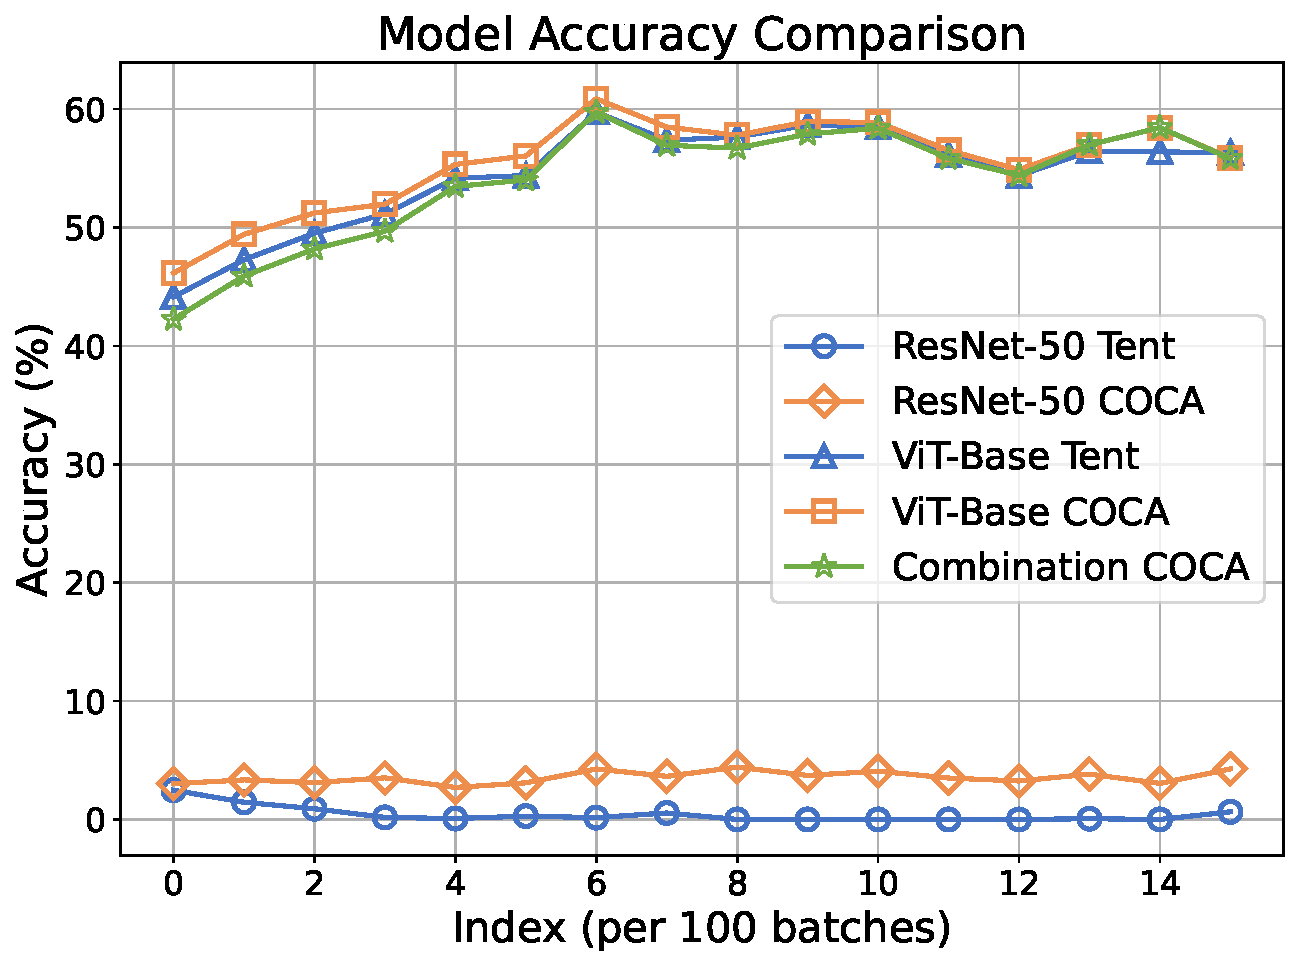
\includegraphics[width=0.85\linewidth]{sec/accuracy_comparison_updated_final.pdf}
    \vspace{-0.12in}
    \caption{Robustness of COCA stems from $\tau$. In the label-shift scenario~\cite{niu2023towards}, COCA maintains high performance even when one of the models—such as ResNet-50 in this figure—collapses. The evaluation is conducted on ImageNet-C with Gaussian noise (\%).} 
    % \vspace{-0.1in}
\label{lsrobust}
\vspace{-0.07in}
\end{figure}

\begin{table}[t]
% \vspace{-0.1in} 
    \centering
    \setlength{\tabcolsep}{9pt} % 调整列间距
    \renewcommand{\arraystretch}{1} % 增加行高(从 1 改为 1.2)
    \begin{threeparttable} % 使用 threeparttable 环境
    \resizebox{0.95\linewidth}{!}{% 
        \begin{tabular}{c|c|cc}
            % \midrule % 增加顶部的横线,使表格更整洁
            Models & \multicolumn{1}{l|}{Accuracy (\%)} & Parameters (M) & GMACs \\
            \midrule
            ResNet-18 & 35.1 & 11.7 & 1.8 \\
            ResNet-50 & 42.9 & 25.6 & 4.1 \\
            ResNet-101 & 46.5 & 44.5 & 7.8 \\
            \midrule
            Mobile-ViT & 41.0 & 10.6 & 4.1 \\
            ViT-Base & 51.7 & 86.6 & 16.9 \\
            ViT-Large & 67.8 & 304.2 & 77.8 \\
            % \midrule % 增加底部的横线
        \end{tabular}%
    }
    \vspace{-0.1in}
    \caption{Comparison of Model Profiles: performance (\%), the number of parameters (in millions), and GMACs. The performance is the average adaptation performance across 15 types of corruption on ImageNet-C, evaluated using Tent ~\cite{wang2020tent}.}
    \label{params}
    \vspace{-0.15in} 
    \end{threeparttable}
\end{table}

\vspace{-5pt}
\paragraph{The Learnable Parameter $\tau$ Enhances the Robustness of COCA}
% In Section 3, we have discussed the necessity of $\tau$, as displayed in Fig.~\ref{Tcompare}. Furthermore, introducing $\tau$ also brings robustness for COCA. In some scenarios, such as label shifts~\cite{niu2023towards}, the ResNet-50-BN model is prone to collapse. Despite this phenomenon, the collaborative model, ViT-Base, can continue to learn effectively, as shown in Fig.~\ref{lsrobust}. The accuracy based on the ResNet-50-BN model is approximately 0, indicating that the predictions of ResNet are very different from ViT. In this condition, the value of $\tau$ will become very large to balance the outputs of the two models. Based on $\tau$, the contribution provided by ResNet to collaborative knowledge computation becomes very small, as illustrated in Eq.~\ref{marginalent}, effectively preventing the impact from being harmful to collaboration since the final performance is near to ViT-Base under COCA. As a result, if one model collapses during cross-model co-learning, we can discard this model and only utilize the adapted predictions of the other model to replace the final performance. 


% In Section.\ref{sec:Method Section}, we discussed the necessity of the parameter $\tau$, as shown in Fig.~\ref{Tcompare}. Additionally, introducing $\tau$ enhances the robustness of COCA. 

As shown in Fig.~\ref{Tcompare} of section.\ref{sec:Method Section}, it is necessary to introduce a learnable parameter $\tau$, which can enhance the robustness of COCA. In certain scenarios, such as label shifts~\cite{niu2023towards}, the ResNet-50-BN model may be prone to collapse. However, in these cases, the collaborative model, ViT-Base, continues to learn effectively, as illustrated in Fig.~\ref{lsrobust}. The accuracy of the ResNet-50-BN model approaches zero, indicating that its predictions diverge significantly from those of ViT. Under such conditions, the value of $\tau$ increases substantially to balance the outputs of the two models. Consequently, the contribution of ResNet-50 to the collaborative knowledge computation diminishes, as shown in Eq.~\ref{marginalent}, thereby preventing any harmful effects on collaboration. This ensures that the final performance remains close to that of ViT-Base under COCA. Therefore, if one model collapses at test time, we can discard it and rely solely on the adapted predictions of the other model to maintain performance. In our experiments, the learnable parameter $\tau$ ranges from 1 to 5. The Appendix~\ref{VisualizeCOCA} further visualizes the benefits of COCA, highlighting how $\tau$ enables robust co-adaptation.

\vspace{-10pt}

\paragraph{Influence of Anchor Model Selection}
The influence of selecting the anchor model is shown in Table~\ref{anchorexchange}, where ``Anc." and ``Aux." refer to the accuracy of the anchor model and the auxiliary model, respectively. We observe that choosing any model as the anchor improves the performance compared to single-model TTA. Additionally, selecting a larger model as the anchor leads to better performance. Notably, the performance gap between the two models increases as the difference in the number of parameters grows. For example, when selecting ViT-Base as the anchor model, the performance is higher than when the auxiliary model is Mobile-ViT, which has fewer parameters than ResNet-50.
\begin{table}[t]
    % \vspace{-0.1in}
    \begin{center}
    \setlength{\tabcolsep}{9pt} % 调整列间距
    \renewcommand{\arraystretch}{1.1} % 增加行高
    \begin{threeparttable}
        \resizebox{\linewidth}{!}{%
            \begin{tabular}{cc|ccc}
Anchor & Auxiliary & Anc. & Aux. & \textbullet~Combined. \\ 
\midrule
ResNet-18 & ResNet-50 & 37.3 & 43.4 & 43.8 \\
ResNet-50 & ResNet-18 & 44.0 & 38.9 & \textbf{45.6} \\ \midrule
ResNet-50 & ViT-Base & 48.5 & 63.0 & 62.2 \\
ViT-Base & ResNet-50 & 63.2&50.7& \textbf{64.9} \\ \midrule
Mobile-ViT & ViT-Base & 47.7 & 63.3 & 61.6 \\
ViT-Base & Mobile-ViT & 64.0& 47.5& \textbf{64.5}
\end{tabular}%
        }
    \end{threeparttable}
    \end{center}
    \vspace{-0.25in}
    \caption{Influence of anchor model selection. Each result represents the average performance across 15 types of corruption on ImageNet-C (\%). It is clear that selecting the larger model as the anchor leads to higher performance.}
    \label{anchorexchange}
    \vspace{-0.15in}
\end{table}





% \paragraph{Effectiveness of Components in COCA }
% In our COCA, we mentioned that naively averaging the outputs combination of two models as collaborative knowledge in collaboration is infeasible, as in Fig.~\ref{Tcompare}, and thus propose a diversity-aware scaling factor $\tau$ to guide effective and stable collaborative learning and boost the adaptation performance. Based  on $\tau$, we construct the separability-enhancing marginal entropy $\mathcal{L}_{mar}$ and cross-model knowledge distillation cross-entropy $\mathcal{L}_{ckd}$. In addition to the collaborative knowledge, we also introduce self-adaptation entropy $\mathcal{L}_{sa}$ to exploit the self-knowledge of each model. We ablate them in Fig.~\ref{Tcompare} and Table.~\ref{ablation}. Firstly, using collaborative knowledge to adapt without $\tau$ performs poorer than each model's self-adaptation following Tent without collaborative knowledge, which verifies the necessity of devising an adaptive scaling factor $\tau$ for integrating collaborative knowledge. Secondly, when applying only $\mathcal{L}_{mar}$ results in 47.9\% accuracy with ResNet-50, 59.9\% with ViT-Base, and 62.5\% with the combined prediction. Meanwhile, applying only $\mathcal{L}_{ckd}$ yields 47.2\% , 59.5\% , and 61.5\% . Each of these outperforms the self-adaptation of the individual models, which suggesting that our collaborative knowledge is working well to provide valuable learning signals to models. Thirdly, Combining $\mathcal{L}_{sa}$ with either $\mathcal{L}_{ckd}$ or $\mathcal{L}_{mar}$ both lead to performance improvements compare to just using $\mathcal{L}_{mar}$ and $\mathcal{L}_{ckd}$, which illustrates the benefits of leveraging self-knowledge for collaboration. Lastly, by incorporating all the three components as the overall fitness function, our COCA achieves the best performance, \textit{i.e.},64,9\% average accuracy of 15 corruptions on ImageNet-C dataset.


% \paragraph{Effects of Anchor Model Selection in COCA} We investigate the impact of choosing different anchor models for co-learning. While selecting a larger model with more parameters might seem intuitive, we also explore the effect of choosing a less optimal anchor. From the results shown in Table.~\ref{anchorexchange}, we have the following observations. 1) Our COCA shows robustness on anchor model's choice, though choosing the models with more parameters generally enhance co-learning performance, when choosing the smaller one still shows improvement compared to using both models independently. For example, the exchange of anchor model identities between ResNet-18 and ResNet-50 resulted in an accuracy impact of 1.8\%. 2) Compared to our anchor mechanism, the pair of Mobile-ViT and ViT-Base collaborate without the anchor mechanism which perform poorer than individual adaptation shown in Fig.~\ref{Tcompare} due to the huge gap between the quantities of two models. However, COCA greatly alleviates this problem by allowing two models with a very large parameter gap to still learn well collaboratively.

% As shown in Table~\ref{anchorexchange}, the results indicate that models with more parameters generally enhance co-learning performance. For example, using ResNet-50 as the anchor model and ResNet-18 as the auxiliary results in 44.0\% accuracy for the anchor, 38.9\% for the auxiliary, and 45.6\% for the combined prediction. However, even when ResNet-18, which has significantly fewer parameters than ResNet-50, is chosen as the anchor, performance still improves compared to using both models independently (see Table.~\ref{params}). Similarly, when ViT-Base and ResNet-50 collaborate, whichever model serves as the anchor leads to better performance than when learning individually (\textit{i.e.} ViT-Base: 57.4\% $\to$ 63.0\% or 63.2\%). These results suggest that while a more powerful anchor model typically yields better performance, collaborative learning remains effective even when the anchor model is suboptimal.



\vspace{-10pt}

% \paragraph{Effectiveness of $\tau$ on robustness in Eq.~\ref{tintro} }
% In collaborative model settings, a key concern is the potential collapse of one model, which could severely disrupt collaboration and degrade overall performance. In the context of Test Time Adaptation (TTA), model collapse is indeed a risk. However, our adaptive scaling temperature mechanism ($\tau$)  effectively mitigates the impact of an auxiliary model's collapse within the COCA framework, helping to preserve the performance of the anchor model. In specific scenarios, such as label shifts introduced by SAR~\cite{niu2023towards}, the ResNet-50-BN model is prone to collapse. Despite this, the collaborative model, ViT-Base, can still continue to learn effectively, as shown in Fig.~\ref{lsrobust}. In this condition, the accuracy of ResNet-50-BN approaches to 0, which indicates the predictions of the ResNet alomst is the opposite of ViT's. At this point, as $\tau$ is learned based on diversity-aware, $\tau$ will rise to a very large value.Then, the contribution provided by ResNet to collaborative knowledge computation will become very small in Eq.~\ref{marginalent}, effectively prevent the impact of collapse model from being harmful to collaboration.

% \vspace{-10pt}


% \begin{table}[t]
%     % \vspace{-0.1in}
%     \begin{center}
%     \setlength{\tabcolsep}{9pt} % 调整列间距
%     \renewcommand{\arraystretch}{1.1} % 增加行高
%     \begin{threeparttable}
%         \resizebox{0.93\linewidth}{!}{
%             \begin{tabular}{cc|ccc}
% Anchor & Auxiliary & Anc. & Aux & \textbullet~Combined \\ \midrule
% ResNet-18\textsuperscript{1} & ResNet-18 & 31.2 & 37.4 & 38.6 \\
% ResNet-18 & ResNet-18\textsuperscript{1} & 37.2 & 31.0 & \textbf{39.9} \\ \midrule
% ResNet-50\textsuperscript{1} & ResNet-50 & 41.7 & 45.8 & 48.5 \\
% ResNet-50 & ResNet-50\textsuperscript{1} & 45.7 & 41.1 & \textbf{49.2}
% \end{tabular}%
%         }
%     \end{threeparttable}
%     \end{center}
%     \vspace{-0.23in}
%     \caption{Investigating whether COCA continues to deliver performance improvements when two models share the same deep architecture but differ in their pre-trained weights. Each result represents the average performance across 15 types of corruption on ImageNet-C (\%). For each pair, the two models have different pre-trained weights. }
%     \label{samemodel}
%     \vspace{-0.1in}
% \end{table}





% \begin{table*}[t]
    
%     \setlength{\tabcolsep}{3pt} % 调整列间距
%     \renewcommand{\arraystretch}{1.0} % 增加行高
    
%     \begin{center}
%     \begin{threeparttable}
%         \resizebox{1.0\linewidth}{!}{%
%             \begin{tabular}{c|ccc|cccc|cccc|cccc|c}
%                 \multicolumn{1}{c}{} & \multicolumn{3}{c}{Noise} & \multicolumn{4}{c}{Blur} & \multicolumn{4}{c}{Weather} & \multicolumn{4}{c}{Digital} &  \\
%                 \midrule
%                 Models & Gauss & Shot & Impul & Defoc & Glass & Motion & Zoom & Snow & Frost & Fog & Brit & Contr & Elastic & Pixel & JPEG & Avg. \\ 
%                 \midrule
%                 Mobile-ViT & 29.7 & 29.0 & 33.2 & 30.1 & 26.5 & 44.8 & 50.9 & 51.3 & 48.0 & 60.8 & 70.0 & 41.9 & 54.0 & 54.6 & 52.1 & 45.1 \\
%                 ResNet-50* & 34.0 & 35.9 & 35.7 & 32.3 & 31.5 & 45.9 & 51.1 & 50.4 & 43.8 & 59.1 & 67.9 & 41.0 & 56.5 & 59.8 & 54.4 & 46.6 \\
%                 \textbullet~Combined & \textbf{37.2} & \textbf{38.1} & \textbf{39.8} & \textbf{35.9} & \textbf{33.7} & \textbf{50.2} & \textbf{55.3} & \textbf{55.6} & \textbf{50.1} & \textbf{63.8} & \textbf{72.3} & \textbf{45.9} & \textbf{59.6} & \textbf{62.1} & \textbf{58.0} & \textbf{50.5} \\
%                 \midrule
%                 ResNet-50 & 34.6 & 37.6 & 36.7 & 32.9 & 32.7 & 47.9 & 52.5 & 51.4 & 41.1 & 59.8 & 67.4 & 22.6 & 57.9 & 60.8 & 55.7 & 46.1 \\
%                 ResNet-101* & 36.0 & 39.2 & 38.2 & 34.8 & 35.4 & 49.3 & 55.1 & 53.2 & 43.1 & 61.3 & 69.6 & 24.5 & 60.3 & 62.5 & 57.7 & 48.0 \\
%                 \textbullet~Combined & \textbf{38.7} & \textbf{41.9} & \textbf{41.0} & \textbf{36.8} & \textbf{37.0} & \textbf{52.4} & \textbf{57.3} & \textbf{55.8} & \textbf{45.1} & \textbf{63.7} & \textbf{71.3} & \textbf{25.6} & \textbf{62.5} & \textbf{65.0} & \textbf{60.1} & \textbf{50.3} \\
%                 \midrule
%                 Mobile-ViT & 32.6 & 34.7 & 35.8 & 33.1 & 32.2 & 46.9 & 50.4 & 54.0 & 51.4 & 61.4 & 70.7 & 46.5 & 55.0 & 55.0 & 53.4 & 47.5 \\
%                 ViT-Base* & \textbf{55.6} & 55.9 & 56.9 & 57.2 & \textbf{55.7} & 62.6 & 58.8 & 65.5 & 64.5 & 73.0 & 78.2 & \textbf{69.8} & 65.6 & 71.2 & 68.7 & 64.0 \\
%                 \textbullet~Combined & 55.2 & \textbf{56.0} & \textbf{57.1} & \textbf{57.3} & 55.6 & \textbf{63.5} & \textbf{61.1} & \textbf{67.3} & \textbf{65.5} & \textbf{73.7} & \textbf{78.8} & 69.0 & \textbf{67.5} & \textbf{71.3} & \textbf{68.8} & \textbf{64.5} \\
%                 \midrule
%                 Mobile-ViT & 31.6 & 34.8 & 35.3 & 32.1 & 32.0 & 47.2 & 51.9 & 53.4 & 50.8 & 61.6 & 70.3 & 45.7 & 55.1 & 55.6 & 53.1 & 47.4 \\
%                 ViT-Large* & 66.0 & 67.4 & 68.2 & 63.6 & 63.4 & 70.4 & 67.9 & 75.8 & 71.6 & 77.4 & \textbf{83.7} & 75.7 & 71.4 & 77.3 & \textbf{75.6} & 71.7 \\
%                 \textbullet~Combined & \textbf{66.4} & \textbf{67.8} & \textbf{68.6} & \textbf{64.0} & \textbf{63.8} & \textbf{70.4} & \textbf{69.0} & \textbf{76.2} & \textbf{72.4} & \textbf{77.8} & 83.4 & \textbf{76.1} & \textbf{72.8} & \textbf{76.8} & 75.2 & \textbf{72.0} \\
%                 \midrule
%                 ResNet-50 & 42.5 & 44.5 & 43.5 & 41.0 & 40.5 & 52.2 & 54.4 & 55.0 & 49.7 & 61.6 & 68.5 & 51.8 & 59.8 & 62.7 & 57.6 & 52.3 \\
%                 ViT-Large* & 66.3 & 67.7 & 68.7 & 63.8 & 64.1 & 70.9 & 68.5 & 76.0 & 71.7 & 77.5 & 83.8 & 76.1 & 71.6 & 77.8 & 75.9 & 72.0 \\
%                 \textbullet~Combined & \textbf{67.1} & \textbf{68.5} & \textbf{69.3} & \textbf{64.8} & \textbf{64.9} & \textbf{71.9} & \textbf{70.2} & \textbf{76.7} & \textbf{72.3} & \textbf{78.2} & \textbf{83.9} & \textbf{76.4} & \textbf{73.6} & \textbf{78.6} & \textbf{76.7} & \textbf{72.9} \\
%                 \midrule
%                 ViT-Base & 58.2 & 58.7 & 59.2 & 59.9 & 58.9 & 64.4 & 60.5 & 66.4 & 64.5 & 73.7 & 78.6 & 71.5 & 66.4 & 72.6 & 70.1 & 65.6 \\
%                 ViT-Large* & 66.4 & 67.5 & 68.4 & 63.8 & 63.8 & 70.5 & 66.6 & 74.3 & 71.6 & 77.1 & 83.7 & 76.1 & 70.3 & 77.4 & 75.6 & 71.5 \\
%                 \textbullet~Combined & \textbf{67.7} & \textbf{68.8} & \textbf{69.4} & \textbf{65.9} & \textbf{65.5} & \textbf{71.7} & \textbf{67.8} & \textbf{74.8} & \textbf{72.4} & \textbf{78.5} & \textbf{83.8} & \textbf{77.3} & \textbf{72.3} & \textbf{78.3} & \textbf{76.1} & \textbf{72.7} \\
%                 \midrule
%             \end{tabular}%
%         }
%     \end{threeparttable}
%     \end{center}
%     \vspace{-0.2in}
%     \caption{The performance of COCA across different model pairs, with results on ImageNet-C (\%). Additional results can be found in Appendix~\ref{allmodelsappendix}.}
%     \label{allmodels}
%     \vspace{-0.1in}
% \end{table*}





\paragraph{Performance Across Different Model Pairs \& Influence of Models' Parameters and Architectures} We first examine the performance of six models under a single-model adaptation framework following Tent~\cite{wang2020tent}, with the results shown in Table~\ref{params}. Next, we form various pairs from these models to further evaluate the applicability of COCA. As presented in Table~\ref{allmodelssup} (cf. Appendix), COCA consistently achieves robust performance across all model pairs, demonstrating that the cross-model co-learning mechanism remains effective even when the paired models share the same architecture, as in the case of ViT-Base and Mobile-ViT. Additionally, under COCA, each model consistently outperforms single-model adaptation following Tent~\cite{wang2020tent}.

From these comparative results, we derive two key insights: (1) models with a larger number of parameters tend to exhibit enhanced performance, and (2) architectural diversity offers additional benefits. Further analysis is provided in Appendix~\ref{MoreAcross}.


% Moreover, COCA remains effective even when the two models share the same deep architecture and differ only in their pre-trained weights. Table~\ref{samemodel} presents results based on ResNet-18 and ResNet-50, demonstrating that the cross-model co-learning mechanism remains robust. In this table, the superscript \textsuperscript{1} indicates that the model was pre-trained on the Instagram-1B hashtag dataset using semi-weakly supervised learning and fine-tuned on ImageNet~\cite{he2016deep}. Models without this superscript were initialized using the pre-trained weights provided by PyTorch. Notably, unlike previous findings, the performance of the anchor model does not consistently outperform that of the auxiliary model.

% \paragraph{Generalization of COCA} COCA focuses on enabling two models to collaborate and learn from each other effectively. To evaluate the generalization performance of the COCA framework, we conducted two experiments: (1) We paired six different models (three CNN-based and three Transformer-based) for collaborative learning to evaluate the improvements across various model combinations. The model profiles and co-learning results are shown in Tables~\ref{params} and \ref{allmodels}. The results demonstrate that COCA consistently improves performance across all model pairs, regardless of whether the models differ in parameter size or share similar architectures. (2) Additionally, we tested COCA with two models that share the same structure but differ in their pre-training strategies on the source domain. The results, presented in Table~\ref{samemodel}, further validate COCA's ability to enable effective co-learning across diverse models. These findings highlight that COCA is a robust and flexible strategy, well-suited for collaborative learning across a wide range of model architectures and training strategies.

\vspace{-10pt}

% \paragraph{Influence of Models' Parameters and Architectures} To further explore the factors influencing COCA's performance, we analyze the impact of model parameters and architectures. The results, summarized in Table~\ref{mainres}, Table~\ref{allmodels}, and Table~\ref{allmodelssup}, lead to the following insights: 1) More parameters enhance performance; 2) Architectural diversity offers benefits. More analysis is presented in appendix. 




% \paragraph{Influence of Models' Parameters and Architectures} To further explore the factors influencing COCA's performance, we analyze the impact of model parameters and architectures. The results, summarized in Table~\ref{mainres}, Table~\ref{allmodels}, and Table~\ref{allmodelssup}, lead to the following insights: 1) More parameters enhance performance. Increasing the parameter count in the auxiliary model enhances overall performance when the anchor model is fixed. For instance, the accuracy improves from 64.9\% with ResNet-50 and ViT-Base to 67.1\% with ResNet-101 and ViT-Base. This improvement is likely because models with more parameters and the same deep architecture can facilitate more comprehensive learning. 2) Architectural diversity offers benefits. Diversity in deep architectures between models improves performance. For pairs of models sharing one common model, the pair with differing architectures outperforms the one with similar parameter sizes but identical architectures. For example, the accuracy of ResNet-18 and ResNet-50 is 45.6\%, while Mobile-ViT and ResNet-50 achieve 50.5\%. This advantage may arise because distinct architectures enable the models to learn more diverse representations from the same source domain. 




% \begin{figure*}[t]
% \centering
%     \includegraphics[width=0.93\linewidth]{sec/samplelevel.pdf}
%     \vspace{-0.1in}
%     \caption{A sample-level analysis highlights the advantages of our proposed cross-model co-learning approach. For each sample, we select the top five predicted probabilities from both ResNet-50 and ViT-Base. However, the final correct prediction, determined by COCA, differs from each of the initial predictions.}
%     % A learnable parameter, $\tau$, is introduced to more effectively ensemble the outputs of the two models. The final predictions, $p_{com}(x)$, are derived from the combined outputs of both models.
%     \vspace{-0.1in}
% \label{samplelevel}
% \end{figure*}

% \vspace{-10pt}
\paragraph{Computational Complexity Analysis} The comparative results in Table~\ref{eff} show that COCA requires similar computational time to Tent~\cite{wang2020tent} and EATA~\cite{niu2022efficient}, while being more efficient than SAR~\cite{niu2023towards} and CoTTA~\cite{wang2022continual}. Notably, unlike CoTTA, which relies on a teacher-student framework, COCA demands less memory and GPU time. This makes COCA particularly useful when GPU resources are limited. In such cases, a smaller model like ResNet-18 can be used in place of a larger model such as ResNet-50. Although the performance may slightly decrease compared to the larger model, it can still yield satisfactory results.



% \paragraph{Ratio Between Co-adaptation and Self-adaptation} The core idea of COCA is bidirectional improvement throughout the entire adaptation process. Additionally, it is designed to be a plug-and-play module, enhancing existing TTA approaches. To keep it as simple as possible, we aim for minimal hyper-parameters. As a result, we set the ratio between co-adaptation and self-adaptation to 1:1. However, as shown in the results for \textit{EATA+COCA(ours)} in Table~\ref{cifar100c}, COCA achieves optimal performance when the ratio is set to 1:2, increasing the accuracy from 69.1\% to 69.5\%, a slight improvement. We believe that setting the ratio in Eq.~\ref{fullloss} to 1:1 represents a trade-off between slightly lower performance, but faster computation, and slightly higher performance, which requires a hyper-parameter that incurs higher computational costs.

% \begin{table}[t]
% \setlength{\tabcolsep}{11pt} % 调整列间距
%     \renewcommand{\arraystretch}{0.9} % 增加行高
% \resizebox{0.95\linewidth}{!}{%
% \begin{tabular}{c|ccc|c}

% \multicolumn{5}{c}{Sample \#1}\\ \midrule \midrule
% Model \textbackslash Class & 98 & 146 & 356 & Predicted class \\ \midrule
% ResNet-50 & 5.4 & 2.1 & 7.5 & 356 (\ding{55}) \\
% ViT-Base & 5.9 & 8.6 & 1.6 & 146 (\ding{55}) \\
% ResNet-50 / $\tau$ & 8.1 & 5.2 & 9.0 & - \\ \midrule
% Combined & 7.0 & 6.9 & 5.3 & 98 (\checkmark)\\ \midrule 
% \multicolumn{5}{c}{Sample \#2} \\ \midrule \midrule
% Model\textbackslash Class & 192 & 334 & 361 & Predicted class \\ \midrule
% ResNet-50 & 8.0 & 6.5 & 4.8 & 192 (\ding{55}) \\
% ViT-Base & 1.6 & 6.9 & 8.0 & 361 (\ding{55}) \\
% ResNet-50 / $\tau$ & 9.8 & 9.7 & 8.2 & - \\ \midrule
% Combined & 5.7 & 8.3 & 8.1 & 334 (\checkmark)
% \end{tabular}%
% }
% \vspace{-0.1in}
% \caption{Further explanation of Fig.~\ref{samplelevel} on how COCA makes accurate predictions for these two samples. The values, all less than 10, represent the predicted logits. }
% \label{Sampleleveltable}
% \vspace{-0.2in}
% \end{table}
% eata 5202 sar 5532 tent 5202 coca1 6574 coca2 10,531 cotta 17,211

\begin{table}[t]
    % \vspace{-0.05in}
    \begin{center}
    \setlength{\tabcolsep}{3pt} % 调整列间距
    \renewcommand{\arraystretch}{1} % 增加行高
    \begin{threeparttable}
        \resizebox{\linewidth}{!}{%
            \begin{tabular}{l|c|cc}
\multicolumn{1}{c|}{Methods} & Accuracy (\%) & GPU Time (s) & Memory Usage \\ \midrule
Source Only & 35.0 & 115 & 1300 \\ \midrule
CoTTA~\cite{wang2022continual} & 56.7 & 724 & 17,211 \\
Tent~\cite{wang2020tent} & 51.7 & 234 & 5202 \\
SAR~\cite{niu2023towards} & 51.9 & 472 & 5532 \\
EATA~\cite{niu2022efficient} & 55.6 & 246 & 5202 \\
DeYO~\cite{lee2024entropy} & 54.1 & 318 & 5371 \\ 
ROID~\cite{marsden2024universal2} & 52.0 & 371 & 7972 \\ \midrule
\textbf{COCA\textsuperscript{1} (ours)}& 56.8 & 315 & 6574 \\
\textbf{COCA\textsuperscript{1} (ours)} +~EATA & \textbf{59.7} & 316 & 6574 \\ \midrule
\textbf{COCA\textsuperscript{2} (ours)}& 58.3 & 317 & 10,531 \\
\textbf{COCA\textsuperscript{2} (ours)} +~EATA & \textbf{60.9} & 319 & 10,531



\end{tabular}%
        }
    \end{threeparttable}
    \end{center}
    \vspace{-0.23in}
    \caption{Computational complexity analysis. COCA¹ and COCA² denote the collaborations between ResNet-18 and ViT-Base, and between ResNet-50 and ViT-Base, respectively. The results are based on ImageNet-C (Gaussian noise).}
    \label{eff}
    \vspace{-0.15in}
\end{table}
% The results are based on ImageNet-C (Gaussian noise). 

\vspace{-7pt}


\paragraph{Rethinking the Advantages of COCA} The consistent superiority of COCA can be attributed to the fact that, when dealing with out-of-distribution data, the two models leverage their unique strengths to collaboratively achieve robust performance. COCA serves as a general framework for cross-model co-learning, allowing a smaller model like MobileViT to effectively guide a larger model like ViT-Base. Furthermore, the co-adaptation between edge models like ResNet-18 and MobileViT surpasses the performance of much larger models such as ResNet-101 (Table~\ref{params}, Table~\ref{allmodelssup} in Appendix), offering valuable insights for tackling resource-constrained tasks. Additionally, COCA updates the parameters of both models simultaneously without causing a significant increase in GPU time (Table~\ref{eff}). 
% —often outperforming that of a larger model
% Additionally, COCA offers a flexible performance-efficiency trade-off by incorporating a smaller auxiliary model like ResNet-18.
\vspace{-7pt}
\paragraph{Is COCA Applicable to More Than Two Models?}
Building on COCA’s mechanism, a new question emerges: Is COCA applicable to multiple models? In particular, can incorporating a third small model further improve the TTA performance? To answer this, we verify our effectiveness across multiple models in Appendix~\ref{suppl:sec:three-models}, which showcases COCA's consistent improvement in overall accuracy with more collaborating models, underscoring our scalability. Results and analyses are detailed in Appendix~\ref{suppl:sec:three-models}.

% Building on COCA’s outstanding performance, a new question emerges: Is COCA applicable to multiple models? In particular, does incorporating a third small model to collaborate with an existing pair of small models further enhance overall performance? We verify our effectiveness across multiple models in Appendix~\ref{suppl:sec:three-models}, which showcases that COCA consistently improves the overall accuracy with more collaborating models. Detailed results and analyses are provided in Appendix~\ref{suppl:sec:three-models}.


% Detailed results and analyses in Appendix provide affirmative answers to both questions.

% The general procedure follows a similar structure to the pseudocode outlined in Algorithm 1 in appendix. Given three models, denoted as M1, M2, and M3, we rank them by size in descending order: M1 $>$ M2 $>$ M3. The co-learning process is conducted in two steps: 1) M2 and M3 are designated as the anchor model and auxiliary model, respectively. COCA is trained using these two models. 2) M1 and the combination of M2 and M3 are designated as the anchor model and auxiliary model, respectively. The detailed results and analysis, proving COCA's applicability to more than two models, are presented in appendix.

% \paragraph{Visualizing the Advantages of COCA} Extensive comparative results demonstrate that COCA consistently outperforms a single model. To further illustrate this advantage, we present two sample cases where, even if individual models make incorrect predictions, their combined output can still yield the correct result. Specifically, we examine Sample 1 and Sample 2 to showcase COCA's benefits. As shown in Fig.\ref{samplelevel}, both the ViT-Base and ResNet-50 models confidently produce incorrect predictions, with the assigned probability for the predicted category significantly higher than for the others. In contrast, our proposed approach, COCA, generates entirely different but correct predictions. Additionally, we use these two samples to explain why COCA can make accurate predictions, leveraging the learnable parameter $\tau$, as detailed in Table\ref{Sampleleveltable}. The combined logit is the average of the logits from ViT-base and the logits from ResNet-50, where the latter is scaled by a factor of $\tau$. Take the predicted logits for category 192 as an example: $5.7 = (1.6 + 9.8) / 2$.
% \vspace{-10pt}


% \begin{table}[h]
% \setlength{\tabcolsep}{11pt} % 调整列间距
%     \renewcommand{\arraystretch}{0.9} % 增加行高
% \resizebox{0.95\linewidth}{!}{%
% \begin{tabular}{c|ccc|c}
% Model\textbackslash Class & 192 & 334 & 361 & Predicted \\ \midrule
% ResNet-50 & 8.0 & 6.5 & 4.8 & 192 (\ding{55}) \\
% ViT-Base & 1.6 & 6.9 & 8.0 & 361 (\ding{55}) \\
% ResNet-50 / $\tau$ & 9.8 & 9.7 & 8.2 & 192 (\ding{55}) \\ \midrule
% Combined & 5.7 & 8.3 & 8.1 & 334 (\checkmark)
% \end{tabular}%
% }
% \caption{Further illustration of sample-level predictions based on the sample's original predicted logits.}
% \label{Sample1}
% \end{table}
% (1) In the collaboration of models, keeping the anchor model unchanged improves performance as the quantity of auxiliary model parameter increases(\textit{i.e.} ResNet-50 + ViT-Base gain 64.9\% combination accuracy $\rightarrow$ ResNet-101 + ViT-Base gain 67.1\% combination accuracy). (2) When models have similar number of parameters, COCA achieves better performance enhancement when the models have different architectures(\textit{i.e.} ResNet-18 + ResNet-50 gain 45.6\% combination accuracy $\rightarrow$ Mobile-ViT+ ResNet-50 gain 50.5\% combination accuracy). In summary, collaborative learning between models with different architectures generally leads to stronger performance, even when their parameter counts are similar, due to the models with different structures learned widely varying knowledge in the source domains. On the other hand, for models with the same architecture, a larger number of parameters typically reflects more comprehensive learning in the source domain, but there is still potential for improvement through collaboration.


% \paragraph{Comparison on Additional Datasets} We also evaluated COCA on two more challenging datasets, ImageNet-R and ImageNet-Sketch\cite{hendrycks2021many}, which involve natural distribution shifts. As shown in Table~\ref{RSdatasets}, COCA consistently delivers significant performance improvements, both when using simple entropy minimization and when combined with other TTA methods. This success can be attributed to COCA's ability to effectively facilitate model collaboration.
 % Acc. (\%, $\uparrow$)
% \paragraph{Comparison with Teacher-Student TTA methods }When it comes to the collaboration of two models in our proposed COCA, the most related framework to us is based on teacher-student network. In recent TTA methods, CoTTA \cite{wang2022continual} use teacher-student networks as the framework for the method. Therefore, we compared COCA with CoTTA, and results are shown in Table. \ref{eff}. From the results, we can see that COCA exhibits significant performance advantages and greatly reduces the cost of memory.
% \vspace{-11pt}\paragraph{Computational Complexity Analysis} In the COCA framework, two models collaborate for adaptation, a concept similar to the teacher-student networks used in recent TTA methods like CoTTA \cite{wang2022continual}.Thus, we compared COCA with CoTTA and other TTA methods, as shown in Table~\ref{eff}. The results demonstrate that COCA not only outperforms CoTTA in terms of adaptation accuracy (58.3\% $vs.$ 56.7\%), but also significantly reduces memory usage, requiring only 11,422 MiB compared to CoTTA's 19,979 MiB. Additionally, COCA achieves this performance with a reasonable computational GPU time of 317 seconds, highlighting its suitability for real-world applications. Moreover, COCA allows for flexibility in model selection, which enabling users to pair different auxiliary models to reduce memory usage without substantial performance degradation (e.g., ResNet-50 + ViT-Base → ResNet-18 + ViT-Base).
% \vspace{-0.35in}


% \textbf{Is COCA applicable on multi-models?} The experimental results indicate that two models can learn from each other and produce better performance. Thus, can more models further increase the performance?
